
\documentclass[a4paper]{article}
\usepackage[left=1in, right=1in]{geometry}
\usepackage{graphicx}
\usepackage[colorlinks=true, urlcolor=blue, linkcolor=red]{hyperref}

\begin{document}

Saagnik Sarbadhikari, 50592327 

Marcus Hartman, 50398874

Bharath Reddy, 50563984

\begin{center}
  Project Phase 1
\end{center}

\begin{enumerate}
  \item Problem Statement (5pts, team)
  
  Title: Forecasting the Rental Housing Economy of Various Areas Using Machine Learning.

  Problem Statement: Develop a model that can accurately predict rent prices across various locations in the next few years. This will use past data along with future predictions on the economy, which can be used by various clients to find the most cost-effective location to rent.

  \bigbreak
  \underline{Potential of the Project}
  
  Explain the potential of your project to contribute to your problem domain. Discuss why this contribution is crucial?

  Our project aims to be useful in multiple aspects of the world. While our project isn't necessarily predicting the outcome of the economy in the next couple of years, we are aiming to get a gauge of the possibilities that the housing economy could take. This contribution aims to prove its usefulness to both current residents and people looking to move into a new area, as they will have a resource at their disposal that could aide in finding the best-fitting place to live a comfortable life economically.

  \item Ask Questions (10pts, individual)
  
  Saagnik:

  \begin{enumerate}
    \item Q1
    \item Q2
  \end{enumerate}

  Marcus:

  \begin{enumerate}
    \item Could there be a larger increase in the gap of rent between a high-income state and one that is lower? Could we see people move to other states to save the money, but work remotely?
    
    \bigbreak
    This is a significant question as it poses a greater risk ever since the rise of remote work. We have seen people already do this, i.e. moving from New York City to Buffalo for this exact reason. I am wondering if this could be seen on a much larger scale, as rent continues to rise in those higher income states.

    \item As rent continues to rise, could we see a decline of these prices to combat multi-family apartments?
    
    The significance of this question arises to illustrate the point of more people opting to live with multiple other people in order to save on rent in smaller buildings. Splitting rent for a three-bedroom apartment between 7 people can be much more affordable than each having their own apartment-- will the market react to this? What would this look like as prices keep rising? This is what an additional hypothesis can be formed to question. The best way to answer this question is to keep track of the price differences between one-bedrooms and multi-bedrooms in the future.
  \end{enumerate}

  Bharath:

  \begin{enumerate}
    \item Q1
    \item Q2
  \end{enumerate}

  \item Data Retrieval (5pts, team)
  
  To help with individual questions that will be asked in Phase 2 and 3, our group has agreed to focus into two states per person. This will make it easier to strike our own findings, and can find different conclusions using the same model.

  \underline{Saagnik:}

  Rural:

  Urban:

  \underline{Marcus:}

  Rural: Minnesota

  Urban: Texas

  \underline{Bharath:}

  Rural:

  Urban:

  \bigbreak
  \begin{center}
    Data Retrieval
  \end{center}

  Sources used (so far):
  \begin{enumerate}
    \item \href{https://www.huduser.gov/portal/datasets/fmr.html#null}{huduser.gov} - $40^{th}$ Percentile Rents (Historic)
    \item \href{https://www.zillow.com/research/data/}{zillow.com} - Current housing markets, estimations for an area
    \item \href{https://www.rentcast.io/api}{rentcast.io} - Additional market data for a zip code area
    \item \href{https://insideairbnb.com/get-the-data/}{insideairbnb.com} - AirBnB rentals by city
  \end{enumerate}

  Data retrieval consists of a couple calls to certain APIs. While the first two sources are free, rentcast unfortunately charges after the $31^{st}$ use of the month. Therefore, we only try to do this call once and store the result in the results/ folder we have for this. 

  The code can be found in the associated ipynb, where the following lines are found: 

  For huduser.gov:

  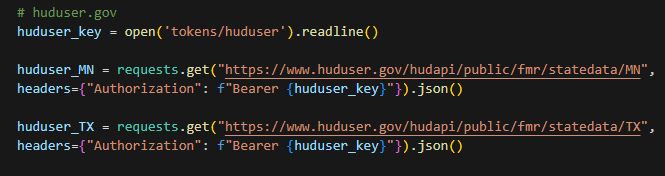
\includegraphics[scale=0.82]{huduser_retrieval.png}

  For zillow.com:

  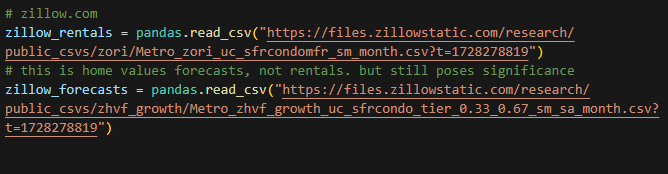
\includegraphics[scale=0.82]{zillow_retrieval.png}

  For rentcast.com:

  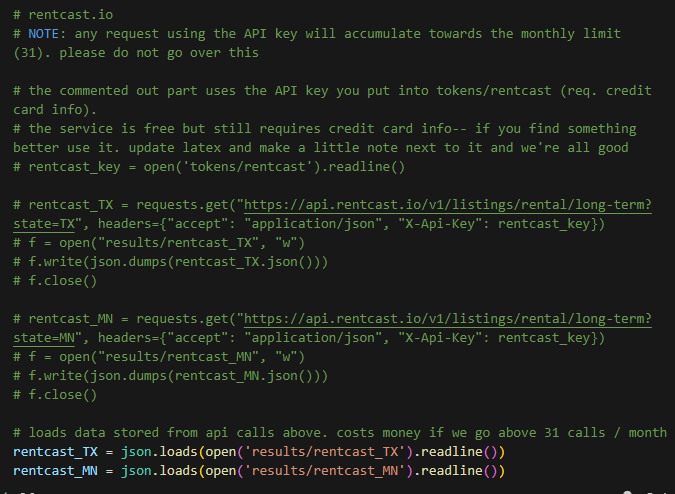
\includegraphics[scale=0.82]{rentcast_retrieval.png}

  For insideairbnb.com:

  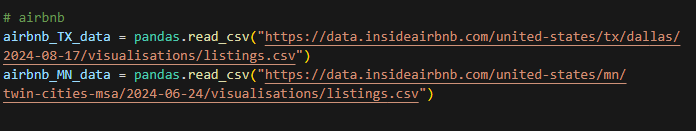
\includegraphics[scale=0.8]{airbnb_retrieval.png}

  \item Data Cleaning (10pts, team)
  
  For each dataset, we cleaned up all of the NaNs, converted every dataset into a similar JSON, and dropped any unnecessary columns pertaining to our problem. Each are separated out by their source.

  For huduser.gov:

  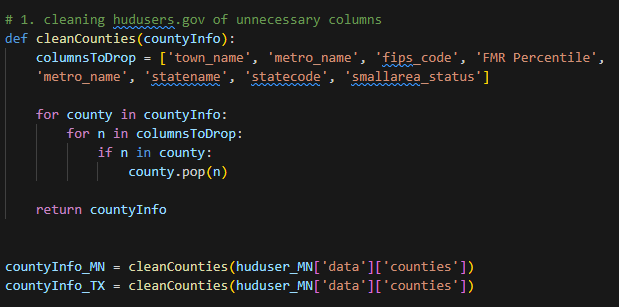
\includegraphics[scale=0.8]{huduser_cleaning.png}

  For zillow.com:

  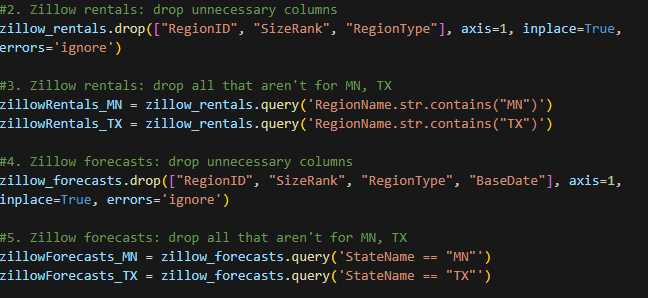
\includegraphics[scale=0.8]{zillow_cleaning.png}

  For rentcast.com:

  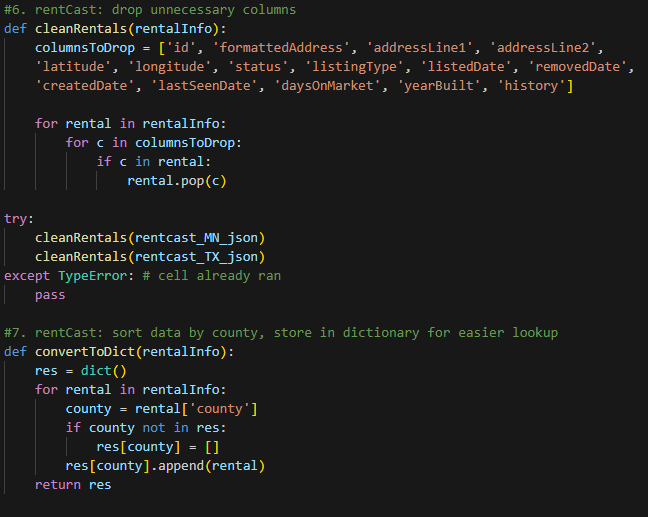
\includegraphics[scale=0.7]{rentcast_cleaning.png}

  For insideairbnb.com:

  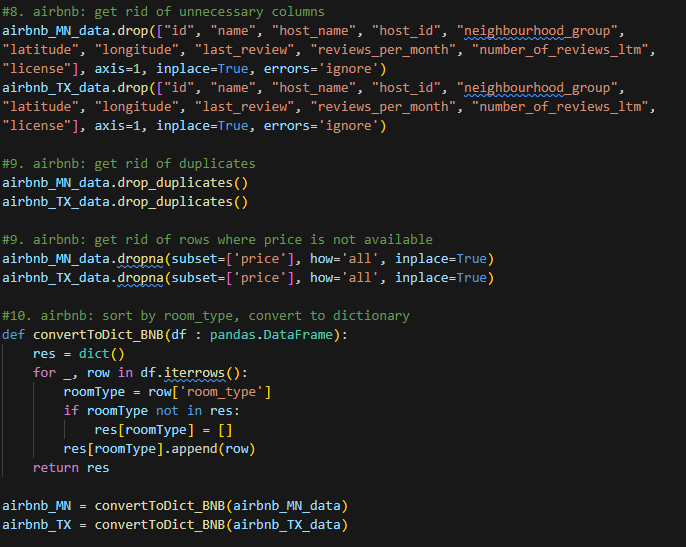
\includegraphics[scale=0.7]{airbnb_cleaning.png}


  \item Exploratory Data Analysis (20pts, individual)
  
  
\end{enumerate}

\end{document}